% !TeX root = ../main.tex
\subsection{Strength Estimation: Development, Estimates, and Evaluation}
\label{sec:strength-development}

The strength model produces a time-indexed distribution of latent ability for each team. Figure~\ref{fig:strength-states} illustrates the output for four teams selected for presentation rather than predictive performance. Each point is a pre-match estimate that excludes the selected match's result and incorporates earlier home and away appearances. The means summarize estimated strength, while the whiskers show marginal uncertainty on the fixed performance-noise scale. These marginal summaries distinguish estimated ability from its uncertainty. The joint model uses the strength-difference mixture in Equation~\ref{eq:difference-mixture}, rather than only the displayed mean and standard deviation.

\begin{figure}[htbp]
\centering
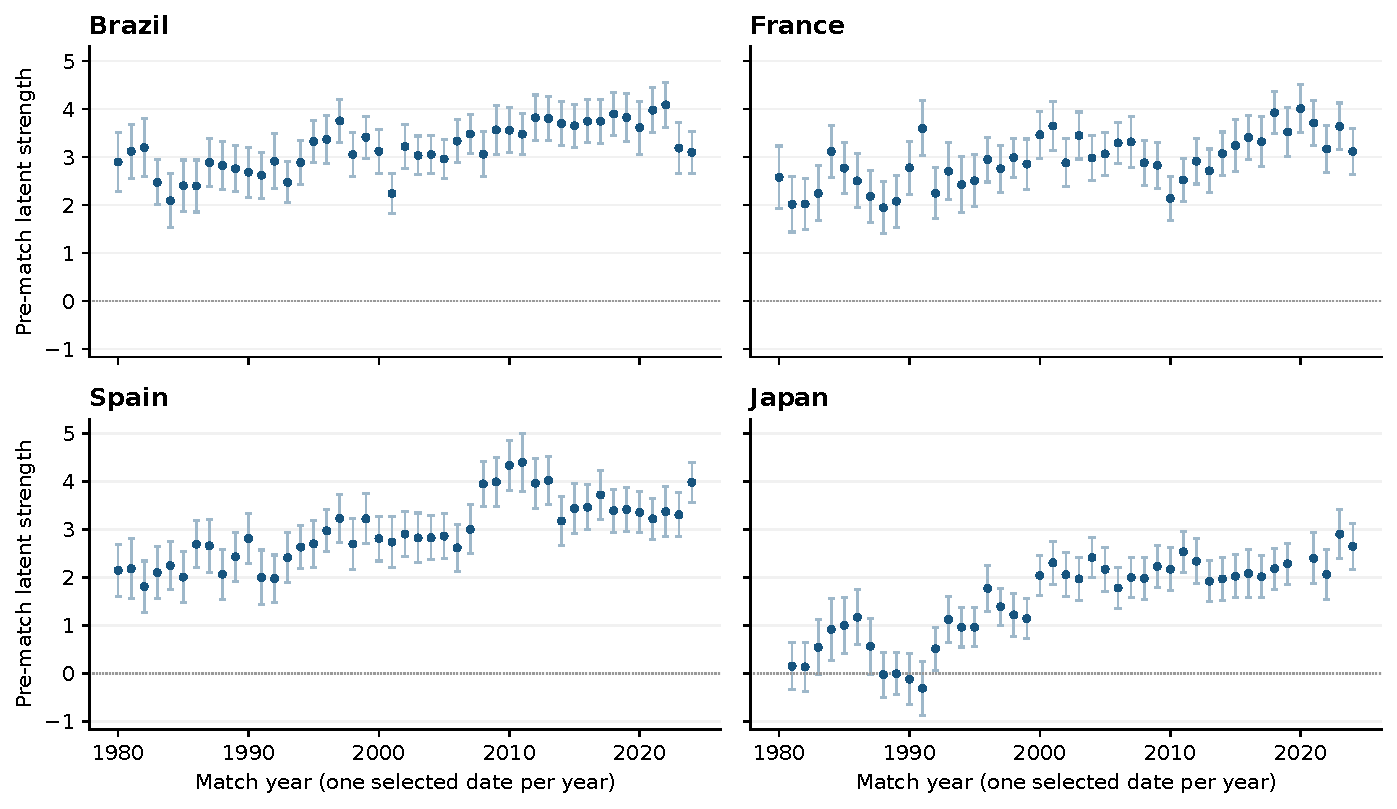
\includegraphics[width=\linewidth]{fig_strength_states.pdf}
\papercaption{Illustrative pre-match strength states, 1980--2024.}{For Brazil, France, Spain, and Japan, each point corresponds to the latest eligible comparative-cohort match in a year, considering both home and away appearances. Whiskers show the marginal mean plus or minus one standard deviation, including jump variance; they do not represent normal-quantile intervals or a world ranking. The zero line is the prior reference. Selected dates do not display every update, and gaps contain no interpolated state estimates.}
\label{fig:strength-states}
\end{figure}

\subsubsection{Model Revisions Informed by Development Results}

Development results informed revisions to the implementation and probability model. They do not establish the optimality of the final rating algorithm. First, explicit expansion of global jump combinations caused excessive memory use. A later moment-collapse approximation still differed from independent numerical references by about $1.328$~pp in match probability, above the original $1$~pp accuracy tolerance. The adopted implementation instead integrates local Poisson counts before processing results, shares a jump variable across a team's same-day matches, and retains the joint covariance. The maximum full-pipeline probability difference between the final ordinary and strict numerical settings was approximately $4.777\times10^{-7}$. This comparison assesses numerical stability for the recorded calculation, rather than the empirical validity of the latent process.

Second, improvements in overall probability scores did not eliminate bias in a particular friendly-match period. Earlier correction candidates underpredicted home wins in the 415 friendlies of 2020--2022 by approximately $3.32$--$4.51$~pp. Separate context fits, switching mixtures, and more flexible matrix corrections did not consistently satisfy the unchanged criteria. Diagnostics indicated distinct errors in probability shape and recent systematic offsets. The final pipeline therefore applies past-only shape correction followed by online residual correction, as described in Section~\ref{sec:strength-method}. For those 415 matches, underprediction decreased to $2.3913$~pp; the corresponding non-friendly bias was $-0.7689$~pp. For 2023--2024, friendly and other-match biases were $+0.9619$ and $+0.3622$~pp. These residual diagnostics do not estimate causal effects of tournament type.

The final comparison included eight candidates, combining two shape mappings with four residual-diffusion values. Two satisfied all prespecified criteria. With diffusion $0.02$, the shared-temperature version had a comparative-cohort loss of $0.890949$, compared with $0.891258$ for the matrix version. These aggregates cover the same 24,917 study matches, not the larger learning population. Candidates were first screened against the criteria, then compared by loss and structural simplicity. The shared-temperature version was selected. The historical data had already been used during development, so these scores do not constitute evaluation on an untouched final holdout. Failed candidates remain documented. The corrections improve the auxiliary probability branch; they do not retrospectively change the strength distributions delivered to the joint analysis.

\subsubsection{Three-Class Evaluation and Remaining Limitations}

Table~\ref{tab:rating-validation} reports the adopted rating-and-correction pipeline on four disjoint historical periods of the comparative cohort. Its target is home win, draw, or away win. The frequency baseline uses earlier venue-specific outcome counts; the internal fixed-step baseline updates both teams from expected-score errors and uses a Davidson-form draw probability. Its registered settings are update size $40$, home offset $100$, and draw parameter $0.75$, on its own rating scale. This internal comparator uses Elo-style updates and is distinct from the official FIFA system. All three issue probabilities before learning the current date's results.

\begin{table}[htbp]
\centering\small
\papercaption{Three-class performance of the final rating pipeline on the comparative cohort.}{The four periods partition 24,917 matches. Loss is three-class negative log probability of the actual result; accuracy selects the most probable of the three outcomes. Bias is predicted minus observed home-win frequency in pp. These results include the probability corrections and reuse development history. They are not directly comparable with the binary scores in Table~\ref{tab:predictive-models}.}
\label{tab:rating-validation}
\begin{tabular*}{\linewidth}{@{\extracolsep{\fill}}lrrrrrr@{}}
\toprule
Period & $n$ & Frequency & Fixed-step & Adopted & Accuracy (\%) & Bias (pp) \\
\midrule
1980--1999 & 8,318 & 1.042385 & 0.939775 & 0.917339 & 56.30 & $+0.1807$ \\
2000--2009 & 6,872 & 1.033723 & 0.895936 & 0.880976 & 59.02 & $-0.0173$ \\
2010--2019 & 6,632 & 1.035877 & 0.880793 & 0.878495 & 60.00 & $+0.0047$ \\
2020--2024 & 3,095 & 1.032750 & 0.863959 & 0.868851 & 60.26 & $-0.3910$ \\
\bottomrule
\end{tabular*}

\end{table}

The pipeline had lower loss than the frequency comparator in every displayed period and lower loss than the fixed-step comparator in the first three. However, in 2020--2024 its loss is $0.868851$ versus $0.863959$, and its accuracy is $60.26\%$ versus $60.97\%$. The loss difference satisfies the prespecified $0.01$ non-inferiority tolerance, although the selected pipeline did not outperform the baseline in every period. The requirements also checked loss improvement of at least $0.005$ against frequency, accuracy no more than $1$~pp below frequency, absolute home-win bias at most $3$~pp, and probability-bin error at most $10$~pp for bins with at least 200 games. Satisfying these tolerances establishes compliance with the operational criteria, rather than general superiority or calibration in every subgroup.

The validation records include 63 targeted tests, independent integration checks, full-history replay, and checkpoint continuation. Simulation under two alternative jump-parameter settings gave nominal $90\%$ strength-difference range coverage of approximately $95.90\%$ and $92.65\%$. These checks assess implementation consistency, numerical approximation, and performance under specified simulation settings. They do not provide observed true-strength labels for real teams. Initialization checks also found 2,905 study matches with a raw home-probability change exceeding $1$~pp under at least one registered alternative, 359 cold starts, and 80 matches whose prior cumulative opponent graph was disconnected. Some match-level initialization effects were substantially larger than the average. The corresponding flags and uncertainty information are retained because a common rating scale does not imply equally reliable comparisons across teams and regions.

The latent strength distributions provide the input to the joint analysis, with the limitations identified above. Corrected three-class probabilities serve as a separate forecasting diagnostic. The common-sample comparison below evaluates the contribution of strength to the binary home-win target and the additional contribution of context.
